%standard 5.1

%start_of_questions


%new_question
%%%%%%%%%%%%%%%%%%%%%
	% Problem 9
	% Difficulty: 1
%%%%%%%%%%%%%%%%%%%%%
	\item
		When driving in a car and approaching a traffic control light, \textit{green} means go, 
		\textit{yellow} means yield, and \textit{red} means stop. Write a \textbf{function} that returns the action 
		that should be taken by a driver. The argument for the function will be 
		$light\_color$ (the current color of the traffic control light).

	\textbf{Examples:}
	\begin{itemize}
		\item  traffic\_light(\csq{red}) $\rightarrow$ \csq{Stop}, 
		\item  traffic\_light(\csq{Green}) $\rightarrow$ \csq{Go}, 
		\item  traffic\_light(\csq{Yellow}) $\rightarrow$ \csq{Yield}
	\end{itemize}


%new_question
%%%%%%%%%%%%%%%%%%%%%
	% Problem 10
	% Difficulty: 1
%%%%%%%%%%%%%%%%%%%%%
	\item
		When using a security access system, different clearance levels are assigned to users. 
		In our system, \textit{admin} means full access, \textit{user} means limited access, 
		and \textit{guest} means view-only access. Write a function named \textbf{access\_rights} 
		that takes user\_role (a string) as an argument and returns the access rights of a user. 

	\textbf{Examples:}
	\begin{itemize}
		\item  access\_rights(\csq{user}) $\rightarrow$ \csq{limited}, 
		\item  access\_rights(\csq{guest}) $\rightarrow$ \csq{view}, 
		\item  access\_rights(\csq{admin}) $\rightarrow$ \csq{full}
	\end{itemize}





%new_question
%%%%%%%%%%%%%%%%%%%%%
	% Problem 11
	% Difficulty: 1
%%%%%%%%%%%%%%%%%%%%%
	\item 
		In Harry Potter, the currency consists of knuts, sickle, and galleon. There are 29 knuts in 
		one sickle and 17 sickles in one galleon. Write a \textbf{function} that will return a 
		converted amount of knuts into the fewest amount of coins possible. Only return a string 
		with the non-zero values, meaning don't return something similar to ``0 sickles''. The 
		argument for the function will be $knuts$ (how many knuts to convert). 

		\textbf{Examples:}
		\begin{itemize}
			\item  convert\_knuts(32) $\rightarrow$ \csq{1 sickle 3 knuts}, 
			\item  convert\_knuts(544) $\rightarrow$ \csq{1 galleon 1 sickles 22 knuts}, 
			\item  convert\_knuts(993) $\rightarrow$ \csq{2 galleons 7 knuts}\\
				Note: Do \textbf{not} output 2 galleons 0 sickle 7 knuts.
		\end{itemize}


%new_question
%%%%%%%%%%%%%%%%%%%%%
	% Problem 12
	% Difficulty: 1
%%%%%%%%%%%%%%%%%%%%%
	\item 
		In an Ancient Kingdom, the currency consists of bronze coins, silver coins, and gold coins.  There are 20 bronze coins in 
		one silver coin and 15 silver coins in one gold coin.  Write a \textbf{function} that will return a converted amount of 
		bronze coins into the fewest amount of coins possible.  Only return a string with the non-zero values, 
		meaning don't return something similar to ``0 silver coins''.  The argument for the function will be 
		$bronze\_coins$ (how many bronze coins to convert). 

		\textbf{Examples:}
		\begin{itemize}
			\item  convert\_bronze(32) $\rightarrow$ \csq{1 silver 12 bronze}, 
			\item  convert\_bronze(544) $\rightarrow$ \csq{1 gold 4 silver 4 bronze}, 
			\item  convert\_bronze(903) $\rightarrow$ \csq{3 gold 3 bronze}\\
				Note: Do \textbf{not} output 3 gold 0 silver 3 bronze.
		\end{itemize}

%new_question
%%%%%%%%%%%%%%%%%%%%%
	% Problem 13
	% Difficulty: 1
%%%%%%%%%%%%%%%%%%%%%
	\item 
		(Game: heads or tails)  Write a \textbf{function} that lets the user guess whether the flip of a coin 
		results in heads or tails. The function randomly generates an integer 0 or 1, which 
		represents head or tail. The function returns if the guess is correct or incorrect. The argument for the function will be $guess$ 
		(the guess of the user, 0 for heads and 1 for tails).\\
		Hint: Use the following lines of code to create the function.
		\begin{verbatim}
		    from random import randint
		    value = randint(0,1) #picks a random integer. Either 0 or 1.
		\end{verbatim}
		\textbf{Examples:}
		\begin{itemize}
			\item  toss\_coin(0) $\rightarrow$ \csq{Correct!} (if the random value is 0) or \csq{Incorrect!} (if the random value is 1), 
			\item  toss\_coin(1) $\rightarrow$ \csq{Correct!} (if the random value is 1) or \csq{Incorrect!} (if the random value is 0) 
		\end{itemize}

%new_question
%%%%%%%%%%%%%%%%%%%%%
	% Problem 14
	% Difficulty: 1
%%%%%%%%%%%%%%%%%%%%%
	\item 
		(Game: Odd or Even)  Write a \textbf{function} that lets the user guess whether a randomly generated number is odd or even. 
		The function randomly generates an integer between 0 and 9 (inclusive) and returns whether the user's guess is correct or incorrect. 
		The argument for the function will be $guess$ (the user's guess, either \csq{odd} or \csq{even}).\\
		Hint: Use the following lines of code to create the function.
		\begin{verbatim}
		    from random import randint
		    value = randint(0,9) #picks a random integer between 0-9 inclusive
		\end{verbatim}
		\textbf{Examples:}
		\begin{itemize}
			\item  guess\_num(\csq{odd}) $\rightarrow$ \csq{Correct!} (if the random value is odd) or \csq{Incorrect!} (if the random value is even), 
			\item  guess\_num(\csq{even}) $\rightarrow$ \csq{Correct!} (if the random value is even) or \csq{Incorrect!} (if the random value is odd) 
		\end{itemize}




%new_question
%%%%%%%%%%%%%%%%%%%%%
	% Problem 16
	% Difficulty: 1
%%%%%%%%%%%%%%%%%%%%%
	\item 
		Primary U.S. interstate highways are numbered 1-99.  Odd numbers (like 5 or 95) go north/
		south, and evens (like 10 or 82) go east/west.  Auxiliary highways are numbered 100-999, and 
		service the primary highway indicated by the rightmost two digits.  Thus, I-405 services 
		I-5, and I-290 services I-90.
		
		Note: 200 is not a valid auxiliary highway because 00 is not a valid primary highway 
		number.\\
		
		Write a \textbf{function} that returns whether the highway runs north/south or east/west or is an invalid highway number. The argument for the function 
		will be $highway\_num$(highway number provided).
		\textbf{Examples:}		
		\begin{itemize}
			\item  highway\_directions(5) $\rightarrow$ \csq{I-5 runs north/south}, 
			\item  highway\_directions(82) $\rightarrow$ \csq{I-82 runs east/west}, 
			\item  highway\_directions(200) $\rightarrow$ \csq{I-200 is an invalid highway number} 
		\end{itemize}

%new_question
%%%%%%%%%%%%%%%%%%%%%
	% Problem 17
	% Difficulty: 1
%%%%%%%%%%%%%%%%%%%%%
	\item 
		Write a \textbf{function} that checks whether a letter is a vowel or consonant.  The function should return \csq{Vowel} if the letter is a vowel and
		\csq{Consonant} if the letter is a consonant. The argument to the function will be $letter$ (a single lowercase letter).\\
		Hint: In the English language, the letters a, e, i, o, and u are the vowels.\\
		\textbf{Examples:}		
		\begin{itemize}
			\item  check\_letter('a') $\rightarrow$ \csq{Vowel}, 
			\item  check\_letter('z') $\rightarrow$ \csq{Consonant}, 
			\item  check\_letter('o') $\rightarrow$ \csq{Vowel} 
		\end{itemize}



%new_question
%%%%%%%%%%%%%%%%%%%%%
	% Problem 18
	% Difficulty: 1
%%%%%%%%%%%%%%%%%%%%%
	\item 
		At the local ice cream store they have 3 flavors, which are Vanilla, Chocolate, and Strawberry.  
		Write a \textbf{function} that returns the selected flavor. If the chosen flavor is not available, let them know.
		The argument to the function will be $selected\_flavor$ (the user's selected flavor).\\
		\textbf{Examples:}		
		\begin{itemize}
			\item  serve\_icecream(\csq{Vanilla}) $\rightarrow$ \csq{Here is your vanilla ice cream!}, 
			\item  serve\_icecream(\csq{Mint}) $\rightarrow$ \csq{Sorry, we don't have mint ice cream.}, 
			\item  serve\_icecream(\csq{Chocolate}) $\rightarrow$ \csq{Here is your chocolate ice cream!} 
		\end{itemize}


%new_question
%%%%%%%%%%%%%%%%%%%%%
	% Problem 19
	% Difficulty: 1
%%%%%%%%%%%%%%%%%%%%%
	\item 
		At the local coffee shop they have 3 types of coffee, which are Espresso, Latte, and Cappuccino.  
		Write a \textbf{function} that returns the selected coffee type. If the chosen type is not available, let them know.
		The argument to the function will be $selected\_coffee$ (the user's selected coffee type).\\
		\textbf{Examples:}		
		\begin{itemize}
			\item  serve\_coffee(\csq{Latte}) $\rightarrow$ \csq{Here is your latte!}, 
			\item  serve\_coffee(\csq{Mocha}) $\rightarrow$ \csq{Sorry, we don't have mocha.}, 
			\item  serve\_coffee(\csq{Espresso}) $\rightarrow$ \csq{Here is your espresso!}
		\end{itemize}



%new_question
%%%%%%%%%%%%%%%%%%%%%
	% Problem 22
	% Difficulty: 1
%%%%%%%%%%%%%%%%%%%%%
	\item 
		%https://edabit.com/challenge/8pDH2SRutPoaQghgc
		Luke Skywalker has friends and family, but he is getting older and having trouble 
		remembering them all.  Write a \textbf{function} that will return the relation defined in the table below.
		The arguments to the function will be $name$ (name of the person related to Luke).\\ 
		\begin{center}
		\begin{tabular}{|l|l|} \hline
			Person 		& Relation \\ \hline \hline
			Darth Vader	& Father \\ \hline
			Leia		& Sister \\ \hline
			Han			& Brother in law\\ \hline
			R2D2		& Droid \\ \hline
		\end{tabular}\\ \hspace*{1in} *If he types any other name, return \csq{unknown}.
		\end{center}
		\textbf{Examples:}		
		\begin{itemize}
			\item  find\_relation(\csq{Darth Vader}) $\rightarrow$ \csq{Father}, 
			\item  find\_relation(\csq{R2D2}) $\rightarrow$ \csq{Droid}, 
			\item  find\_relation(\csq{Jabba the Hutt}) $\rightarrow$ \csq{Unknown}
		\end{itemize}


%new_question
%%%%%%%%%%%%%%%%%%%%%
	% Problem 23
	% Difficulty: 1
%%%%%%%%%%%%%%%%%%%%%
	\item 
		Detective Sherlock Holmes is solving cases, but he sometimes forgets the key suspects in his investigations. 
		Write a \textbf{function} that will return the suspect defined in the table below.
		The arguments to the function will be $name$ (name of the suspect).\\ 
		\begin{center}
		\begin{tabular}{|l|l|} \hline
			Person 		& Role \\ \hline \hline
			Moriarty	& Archenemy \\ \hline
			Watson		& Best Friend \\ \hline
			Mrs. Hudson			& Landlady \\ \hline
			Inspector Lestrade		& Detective \\ \hline
		\end{tabular}\\ \hspace*{1in} *If he types any other name, return \csq{unknown}.
		\end{center}
		\textbf{Examples:}		
		\begin{itemize}
			\item  find\_relation(\csq{Moriarty}) $\rightarrow$ \csq{Archenemy}, 
			\item  find\_relation(\csq{Mrs. Hudson}) $\rightarrow$ \csq{Landlady}, 
			\item  find\_relation(\csq{Mycroft Holmes}) $\rightarrow$ \csq{Unknown}
		\end{itemize}



%new_question
%%%%%%%%%%%%%%%%%%%%%
	% Problem 24
	% Difficulty: 1
%%%%%%%%%%%%%%%%%%%%%
	\item 
		Write a \textbf{function} that loops through a word and prints every other letter of the word starting with the \textbf{second} letter.
		The argument to the function will be $word$ (the word to loop through and output every other letter).

		\textbf{Examples:}		
		\begin{itemize}
			\item  skip\_letter(\csq{counterattack}) $\rightarrow$ \csq{oneatc}, 
			\item  skip\_letter(\csq{banana sunday}) $\rightarrow$ \csq{aaasna}
		\end{itemize}

%new_question
%%%%%%%%%%%%%%%%%%%%%
	% Problem 25
	% Difficulty: 1
%%%%%%%%%%%%%%%%%%%%%
	\item 
		Write a \textbf{function} that loops through a word and prints every other letter of the word starting with the \textbf{first} letter.
		The argument to the function will be $word$ (the word to loop through and output every other letter).

		\textbf{Examples:}		
		\begin{itemize}
			\item  skip\_letter(\csq{counterattack}) $\rightarrow$ \csq{cutrtac}, 
			\item  skip\_letter(\csq{banana sunday}) $\rightarrow$ \csq{bnnsna}
		\end{itemize}


%new_question
%%%%%%%%%%%%%%%%%%%%%
	% Problem 28
	% Difficulty: 1
%%%%%%%%%%%%%%%%%%%%%
	\item 
		Write a \textbf{function} that creates a word one letter at a time until the 
		user types done, and returns the newly created word. There are no arguments to 
		this function. 	You may name the function $create\_word()$.

		\textbf{Examples:} \\
		 \begin{center}
		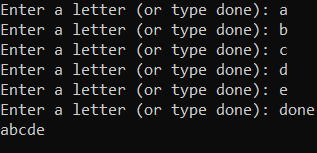
\includegraphics[width = 2.5in]{./imgs/lettersAbcde.PNG} \hspace{0.5in} 
		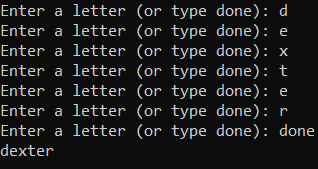
\includegraphics[width = 2.5in]{./imgs/lettersDexter.PNG}
		\end{center}


%new_question
%%%%%%%%%%%%%%%%%%%%%
	% Problem 29
	% Difficulty: 1
%%%%%%%%%%%%%%%%%%%%%
	\item 
		Write a \textbf{function} that sums up integers until a negative integer is given 
		and then returns the sum.
		There are no arguments to this function. You may name the function $sum\_loop()$.

		\textbf{Examples:} \\
		 \begin{center}
		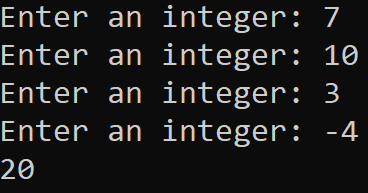
\includegraphics[width = 2.5in]{./imgs/AddCalc2.PNG} \hspace{0.5in} 
		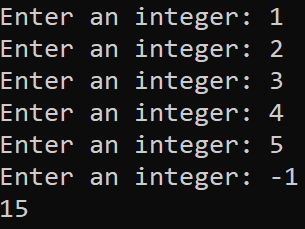
\includegraphics[width = 2.5in]{./imgs/AddCalc1.PNG}
		\end{center}

%new_question
%%%%%%%%%%%%%%%%%%%%%
	% Problem 30
	% Difficulty: 1
%%%%%%%%%%%%%%%%%%%%%
	\item 
		Given a positive integer $n$, the following rules will always create a sequence that 
		ends with 1, called Hailstone Sequence:
		\begin{enumerate}
			\item If $n$ is even, divide by 2
			\item If $n$ is odd, multiply by 3 and add 1 (i.e. $3n+1$)
			\item Continue until $n$ is 1
		\end{enumerate}
		Write a \textbf{function} that returns the hailstone sequence starting at $n$. 
		The argument to the function will be $n$ (the integer to start the sequence from).
		\textbf{Examples:}		
		\begin{itemize}
			\item  hailstone\_seq(25) $\rightarrow$ 25, 76, 38, 19, 58 ... 8, 4, 2, 1, 
			\item  hailstone\_seq(40) $\rightarrow$ 40, 20, 10, 5, 16, 8, 4, 2, 1
		\end{itemize}



%new_question
%%%%%%%%%%%%%%%%%%%%%
	% Problem 31
	% Difficulty: 1
%%%%%%%%%%%%%%%%%%%%%
	\item 
		%https://edabit.com/challenge/6Pf5GGG6HnzbB95gf
		Write a \textbf{function} that returns the factors of a given integer. The argument of the function
		will be $num$ (integer to find factors for).

		\textbf{Examples:}		
		\begin{itemize}
			\item  find\_factors(12) $\rightarrow$ 1, 2, 3, 4, 6, 12, 
			\item  find\_factors(17) $\rightarrow$ 1, 17,
			\item  find\_factors(36) $\rightarrow$ 1, 2, 3, 4, 6, 9, 12, 18, 36
		\end{itemize}



%new_question
%%%%%%%%%%%%%%%%%%%%%
	% Problem 33
	% Difficulty: 1
%%%%%%%%%%%%%%%%%%%%%
	\item 
		%https://edabit.com/challenge/aqDGJxTYCx7XWyPKc
		Write a \textbf{function} that returns the sum of the squares of all positive integers up to a given integer (inclusive). The
		argument to the function will be $num$ (the number up to which squares should be summed).
 
		\textbf{Examples:}		
		\begin{itemize}
			\item  square\_sum(3) $\rightarrow$ 14 ($1^2 + 2^2 + 3^2 = 14$)
			\item  square\_sum(8) $\rightarrow$ 204 ($1^2+2^2+3^2+4^2+5^2+6^2+7^2+8^2=204$)
			\item  square\_sum(-3) $\rightarrow$ \csq{unknown}
		\end{itemize}


%new_question
%%%%%%%%%%%%%%%%%%%%%
	% Problem 34
	% Difficulty: 1
%%%%%%%%%%%%%%%%%%%%%
	\item 
		Write a \textbf{function} that returns the sum of the cubes of all positive integers up to a given integer (inclusive). The
		argument to the function will be $num$ (the number up to which cubes should be summed).

		\textbf{Examples:}		
		\begin{itemize}
			\item  cube\_sum(3) $\rightarrow$ 36 ($1^3 + 2^3 + 3^3 = 36$)
			\item  cube\_sum(8) $\rightarrow$ 1296 ($1^3+2^3+3^3+4^3+5^3+6^3+7^3+8^3=1296$)
			\item  cube\_sum(-3) $\rightarrow$ \csq{unknown}
		\end{itemize}


%end_of_questions
%make sure to leave at least one blank line below

